\section{CAnalytics Features}\label{canalytics-features}

\begin{figure*}
	\centering
    \label{fig:interface}
	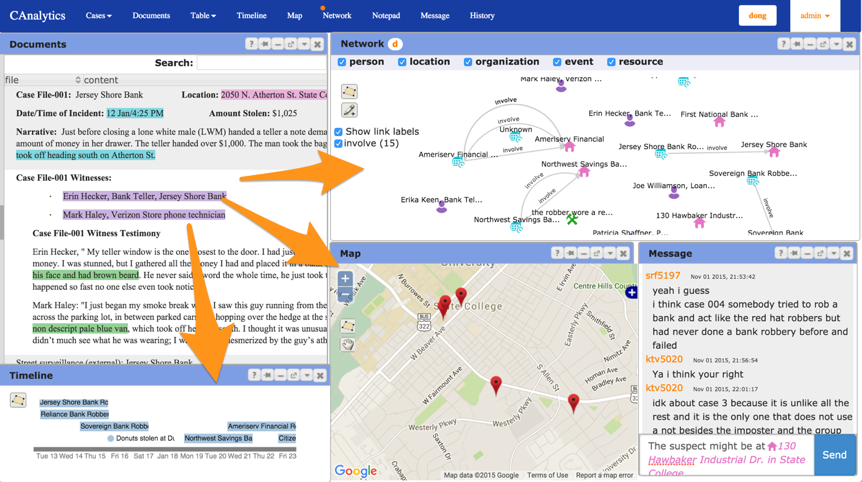
\includegraphics{./img/interface.png}
	\caption{CAnalytics user interface}
\end{figure*}

We developed a collaborative information analysis tool, CAnalytics (Figure~\ref{fig:interface}), to
support teams of analysts in identifying, visualizing, integrating and
assessing facts from multiple sources. The design is informed by our
paper prototype studies, where we examined communication patterns and
team's spontaneously created artifacts when teams were engaged in a
complex crime scenario. We also take into account findings from
empirical studies conducted by Chin et al. \autocite{Chin2009} and Kang
and Stasko \autocite{Kang2011} when making design decisions.

CAnalytics supports evidence modeling through annotation. In the
document view users can select and highlight snippets of information and
annotate them as a type of entity such as a person, location, events,
etc., or as a relationship between entities. Unlike in other
entity-based systems such as \autocites{Bier2010}{Stasko2008}, in which
natural language processing (NLP) techniques are employed to extract and
model entities automatically, we use annotation to allow analysts to
manually create evidence objects of interest. While algorithms for named
entity recognition have improved significantly, developers of the
entity-based systems (e.g. \autocite{Gorg2014}) admitted that the
accuracy of automatic entity extraction is not sufficient to support
human analysis. Besides, relationships identified by algorithms are
limited to co-occurrence of entities in the same document, whereas
identifying meaningful relationships \emph{implicit} in documents that
are of more importance to analysts is not possible. And perhaps the most
problematic is the fact that the NLP treats all pieces of information
equally with no regard to the problem analysts have at hand. We posit
that information analysis is a progressive process, wherein analysts
place varying priority on evidence depending on how they frame the
problem \autocite{Heuer1999}. Manual annotation allows for greater user
control, allows more integrated source data objects to be identified,
and avoids the user problems associated with automatic identification of
disaggregated people, locations and times \autocite{Bier2008}.Users can
decide their own information of interest and granularity that best suits
their ad-hoc analytic needs.

Users can add attributes to the annotated object, e.g.~adding time
attribute in an event, and placing coordinate in a location. Users can
also make reference to other objects in the attribute; for example,
users can add people objects to an event indicating that these people
were involved in the event. In this case, a relationship between the
people and the event is automatically created. Users can also explicitly
create a relationship between two entities by selecting a source entity
and a target entity and labeling the relation name.

When users are explicitly creating an annotation, they are also
implicitly creating a provenance of the modeled entity--- annotation
records the source where a data object was created. As observed in
Carroll et al.'s \autocite{Carroll2013} empirical study, while
integrating information in a visual artifact helps sharing and pooling
information with teammates, the action also removes problem information
from its original context. Participants often forget what an entity
refers to and why it is such positioned in an artifact. Entities in
CAnalytics are linked back to the location of documents where they were
created through annotation. Users can always re-access the data objects
for provenance, a critical requirement emphasized by Chin et al.
\autocite{Chin2009}.

The data modeled through annotation is then displayed in multiple
coordinated views in the same workspace, including table, timeline, map,
and network graph---artifacts frequently constructed to hold attribute
data, temporal data, spatial data and relational data respectively
\autocite{Carroll2013}. Figure~\ref{fig:interface} shows an example of the tool interface:
when an annotation is created in the document view with information
about time, location, participants, and their relationships, a new event
is created in the timeline view, a new location is created in the map
view, and new people are added to the network graph with a labeled edge
representing the relationship (or new edges are added to existing
nodes). Hovering mouse over an entity will activate an entity detail
window that displays attributes in detail, and analysts can modify, or
re-model the entity in situ.

The views are coordinated and afford brushing and linking interaction;
that is, when users apply a graphic filter in one view, related
information is displayed in other views. Thus the analyst can retrieve
entities within a time range using timeline filter, make a spatial query
with map filter, or select a cluster of entities by drawing a filter
area in the network view.

CAnalytics supports real-time collaborative editing, similar to the
Google Tools. Users can open several concurrent editors to
collaboratively edit multiple annotations. Annotations are immediately
shared within a team and are automatically added to teammates' document
views and other visualizations. As far as we know, this tool is the
first to support multi-concurrent editing, which we think can improve
fine grain coordination and awareness in complex collaborative work.

In addition to real-time data sharing, CAnalytics is built in with
several other awareness features, including a notification system, a
feature we named ``tool coordinator'`, a message tool, and a history
tool, and a collaborative editor. A notification system sends
individual's actions to the team, in the form of a text box in the top
right corner of the workspace. The tool coordinator is an iconic
indicator on top of a tool window, suggesting who is working on the
tool. The message tool is a real time chat window that enables team
communication with persistent message history. The system also maintains
a traceable log of time-stamped individual activities in a history tool.
Users can learn team activity about who did what to which object at
when. Entities and relationships mentioned in the message tool and
history tool are hyperlinks that will trigger pop-up detail window when
being moused over. With these awareness features, users who work
synchronously can be informed of others' activity continuingly; users
who work asynchronously will be able to use the history to reconstruct
their work status and become aware of changes beyond the point of their
last interaction.

We also included a simple notepad to support collaborative hypothesis
development. We integrated Etherpad \footnote{http://etherpad.org}, an
open-source collaborative editor similar to Google Doc, for teams to
compose their hypotheses. Users can insert tables (e.g.~an ACH matrix)
and images (e.g.~screenshots of the tool views).
